% One-pager on Experiment 4b (controlled difference with the capital as the final token): conclusion first, two figures.
% Run results/20261024-150407_exp4cap (random-final-token comparison: results/20261024-000548_exp4ctrl, exp4_onepager.pdf).
% Figures from ../exp4/onepager_capital_figures.py; wording follows the adversarial verification (exp4/LOG.md).
% Build (from this folder): pdflatex exp4b_onepager.tex
\documentclass[10pt]{article}
\usepackage[letterpaper,hmargin=0.5in,vmargin=0.32in]{geometry}
\usepackage[T1]{fontenc}
\usepackage[scaled=0.92]{helvet}
\renewcommand{\familydefault}{\sfdefault}
\usepackage{microtype}
\usepackage{xcolor}
\usepackage{graphicx}
\usepackage{enumitem}
\usepackage[hidelinks]{hyperref}
\setlength{\parindent}{0pt}
\setlength{\parskip}{2pt}
\setlist{nosep,leftmargin=1.2em,itemsep=1.5pt}
\definecolor{cblue}{HTML}{2A78D6}
\definecolor{corange}{HTML}{EB6834}
\definecolor{ink2}{HTML}{52514E}
\definecolor{muted}{HTML}{898781}
\definecolor{axis}{HTML}{C3C2B7}
\definecolor{plane}{HTML}{F4F3EF}
\definecolor{wordbg}{HTML}{DCEAFB}

% token chips: \tb BOS, \tk random filler, \tw inserted word, \tq final token (where attention is measured)
\newcommand{\chip}[3]{{\setlength{\fboxsep}{1pt}\setlength{\fboxrule}{0.4pt}\fcolorbox{#1}{#2}{\strut\ttfamily\footnotesize #3}}\hspace{0.8pt}}
\newcommand{\tb}{\chip{ink2}{ink2}{\color{white}BOS}}
\newcommand{\tk}[1]{\chip{axis}{white}{\color{muted}#1}}
\newcommand{\tw}[1]{\chip{cblue}{wordbg}{#1}}
\newcommand{\tq}[1]{\chip{corange}{white}{\bfseries #1}}
\newcommand{\gap}[1]{{\color{muted}\footnotesize\,\dots\,#1\,\dots\,}}
\newcommand{\ex}[1]{\leavevmode\makebox[1.75cm][l]{\color{ink2}\small\bfseries #1}}
\newcommand{\head}[2]{\par{\large\bfseries #1}\hfill{\color{muted}\footnotesize #2}\\[-3pt]\rule{\linewidth}{0.5pt}\par}

\begin{document}

{\LARGE\bfseries With its capital at the end, GPT-2 finds the country anywhere and rests less}\\[3pt]
{\small\color{ink2} GPT-2 small, 200 random rows $\times$ 11 country--capital pairs per filler type. The final token $T$ is
the country's capital, the same in both versions of each pair. The versions differ only at position $\tau$: the country, or
the row's own token. $\Delta$ = attention from $T$ to $\tau$, country $-$ original, at every distance $T-\tau = 1\ldots31$.
Control: the same with a wrong capital at $T$ (France \dots\ Tokyo).}\\[2pt]
\ex{original}\tb\tk{she}\tk{sc}\gap{26 random tokens}\tk{age}\tk{dis}\tq{Paris}\hspace{1.2em}%
\ex{country}\tb\tk{she}\tk{sc}\gap{26 random tokens}\tw{France}\tk{dis}\tq{Paris}\hspace{0.5em}{\footnotesize\color{muted}($\tau$ = 30, distance 2)}

\vspace{4pt}
\colorbox{plane}{\parbox{\dimexpr\linewidth-2\fboxsep}{\small
\textbf{Conclusion} {\footnotesize\color{muted}(common / rare filler)}
\begin{itemize}
\item \textbf{The matching capital lowers late-layer resting at every distance.} Late (layers 6--11) attention on BOS drops by
  \textbf{0.031 / 0.017} at distance 1 and by 0.033 / 0.028 at distances 16--31, against a wrong capital. It needs the country
  (a placebo word gives $\approx 0$), and the freed attention does not go to the country. It holds for 10 of the 11 pairs; Canada is the exception.
\item \textbf{Early heads link same-country tokens at any distance.} With its own capital at $T$, L0H2 puts \textbf{0.43 / 0.40}
  of its attention on the country (0.38 / 0.35 twenty tokens back), against 0.03 with a wrong capital. L4H10, L3H0 and L1H11 do the same.
  They are not specific to ``capital of'': demonyms, non-capital cities and the reverse direction work too. In layer 0 this is a
  fixed token-pair association.
\item \textbf{The advisor's L11H8 is boosted by a place-name query, not by the fact.} Its $\Delta$(1) is +0.160 / +0.071 with its
  capital, the same with a wrong capital, and +0.065 / +0.039 with a random token. A non-capital city boosts it as much.
\item \textbf{Previous-token heads look away from an adjacent same-country token}, toward the capital itself and the token two back.
  For example, L3H7 drops from 0.51 to 0.24 on France, and even L4H11 drops from 0.98 to 0.91 / 0.86.
\end{itemize}}}

\vspace{4pt}
\head{1 \textperiodcentered\ Four heads, three final tokens}{top: common filler; bottom: rare; grey band = $|\Delta| < 0.02$}
{\centering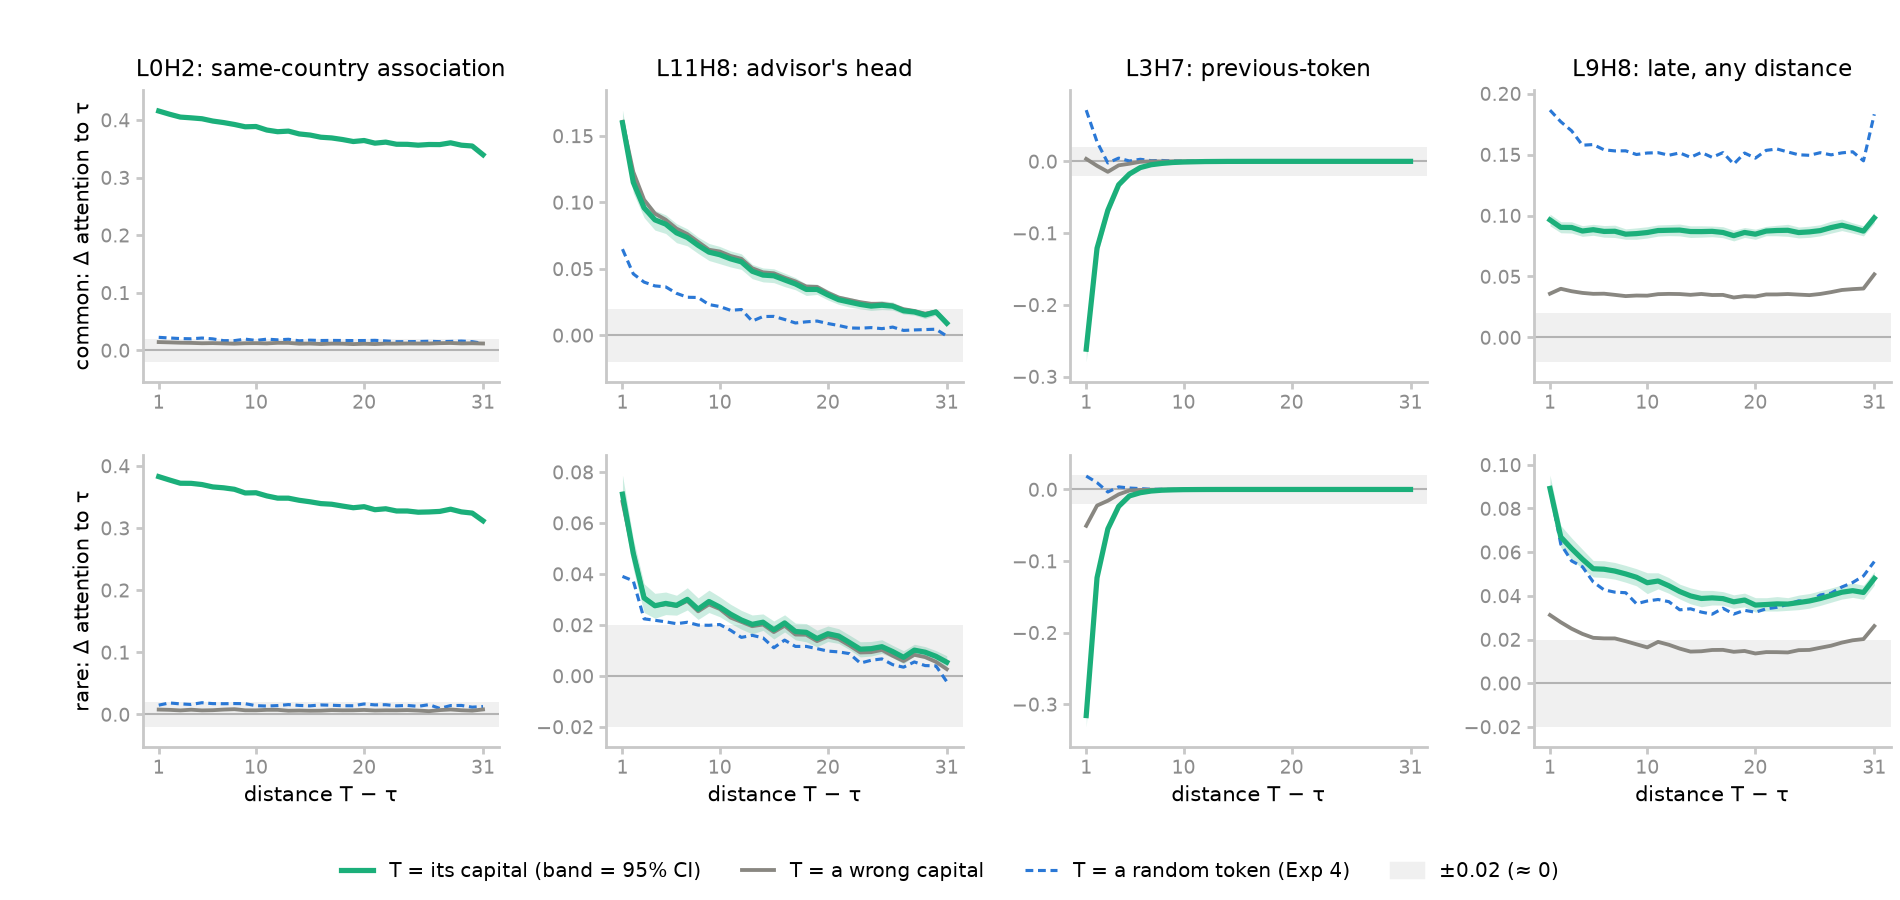
\includegraphics[width=0.86\linewidth]{exp4b_heads.png}\par}
{\small L0H2: only the matching capital, flat with distance. L11H8: any capital. L3H7: drops only for a matching adjacent country.
L9H8: a wrong capital suppresses it (a random final token gives as much or more).\par}

\vspace{4pt}
\head{2 \textperiodcentered\ Where the matching capital matters}{dots = BH $q \le 0.05$ and $|\Delta| \ge 0.02$}
{\centering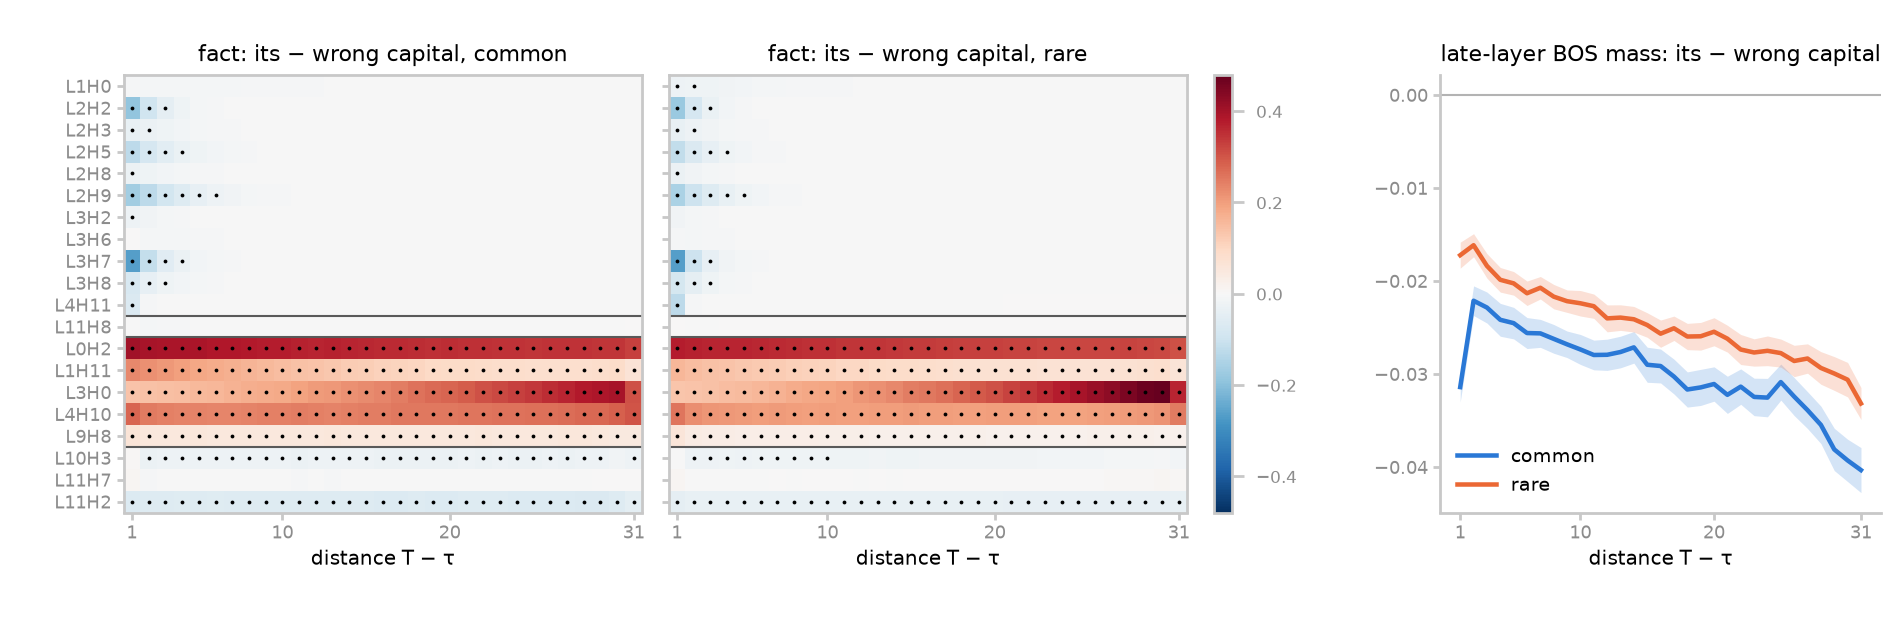
\includegraphics[width=0.9\linewidth]{exp4b_fact.png}\par}
{\small Rows: previous-token heads; L11H8; same-country heads and L9H8; L10H3, L11H7, L11H2. L11H2 and, more weakly, L10H3
attend \emph{less} to the country under its own capital.\par}

\vfill
{\footnotesize\color{muted} Pre-registered (exp4/PREDICTIONS\_capital.md): F1, F2 and F5 pass. F3, F4 and F6 fail, F6 narrowly
(L1H0 at distance 9). All checks pass, and an independent recomputation matched. Probes: 30 rows. Random final token:
exp4\_onepager.pdf. Interactive:
\href{https://pleyva2004.github.io/MechInterp/no-op-research/Experimen_1_Refactored/onepager/exp4_slider.html}{country slider},
\href{https://pleyva2004.github.io/MechInterp/no-op-research/Experimen_1_Refactored/onepager/exp4_viewer.html}{per-head viewer}.}
\end{document}
